\documentclass[10pt]{article}
\usepackage[top=1in, bottom=1.25in, left=1in, right=1in]{geometry}
\usepackage{amsmath}
\usepackage{amssymb}
\usepackage{enumitem}
\usepackage{graphicx}


\usepackage{fancyhdr}
\pagestyle{fancy}
\lhead{MATH7241: Project Report}
\rhead{David Zhao\\Benjamin Quiring\\\today}
\setlength{\headheight}{40pt}

\newcommand{\solution}{\textbf{Solution. }}
\newcommand{\deff}{\underline{Def. }}
\newcommand{\thm}{\underline{Theorem. }}
\newcommand{\lemma}{\underline{Lemma. }}
\newcommand{\corollary}{\underline{Corollary. }}
\newcommand{\proof}{\emph{Proof }}

%\newenvironment{proof}{\par\noindent{\it Proof.}\hspace*{1em}}{$\Box$\bigskip}

\setlength{\parindent}{0em}
\setlength{\parskip}{0.5em}
\begin{document}
\section{Data}
We downloaded a history of terminal commands for a UNIX computer from Perdue
back in 1998. A sample of the data looked like:
\begin{verbatim}
cd
<1>
ll
vi
<1>
ll
emacs
\end{verbatim}

Where a \texttt{<\#>} represents the number of arguments given to a command.
This was done to preserve the user's privacy. We cleaned the data as follows:
\begin{enumerate}
  \item We combined a command with the number of arguments passed with it. For
    example \texttt{cd<1>} is different from \texttt{cd} which is also different
    from \texttt{cd<2>}.
  \item We ignored operators like \texttt{; , -, |} and didn't consider them
    commands.
  \item We ignored the \texttt{**SOF**} and \texttt{**EOF**} commands because
    they were added and not actually typed by the user.
\end{enumerate}

After cleaning up the data as described above, we noticed that there were over
$700$ unique commands. We chose the $28$ most common occuring commands to be the
states in our Markov chain and proceeded to further filter the data by deleting
commands that are not the $28$ most common. The resulting dataset contained only
the top $28$. In order to preserve some semblance of the chain, if there was a
sequence $Y \rightarrow X_1 \rightarrow ... \rightarrow X_n \rightarrow Z$ with $Y$ and $Z$ in the top $28$ and $X_1, ..., X_n$ not, then this reduced to
$Y \rightarrow Z$; i.e. we tried to keep edges. If we did not do this, then we would just have very strange fragments (and the plot of the chain would not work).
Although it loses information, it seems to work pretty well.

Additionally, there were nine different users (two were the same person, but different machines).
Since each person uses different commands (different preferences in text editors,
as well as different alias's for commands). We ended up choosing the user with the most
data and ignored the rest, as that would not really be a Markov process.

There were over twenty thousand time steps in the filtered data, which should be enough to have a meaningful chain.

\begin{figure}[!htb]
  \centering
  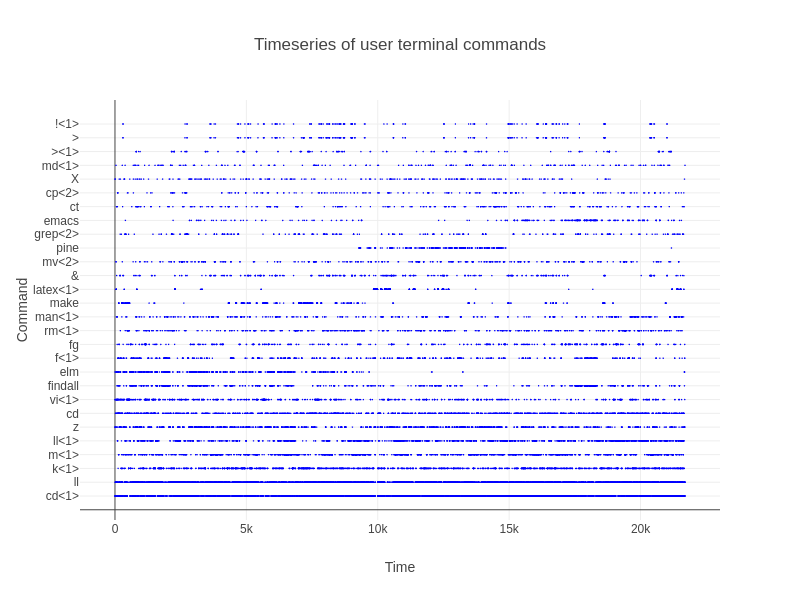
\includegraphics[scale=.47]{../pictures/complete-empirical-timeseries.png}
\end{figure}

\begin{figure}[!htb]
  \centering
  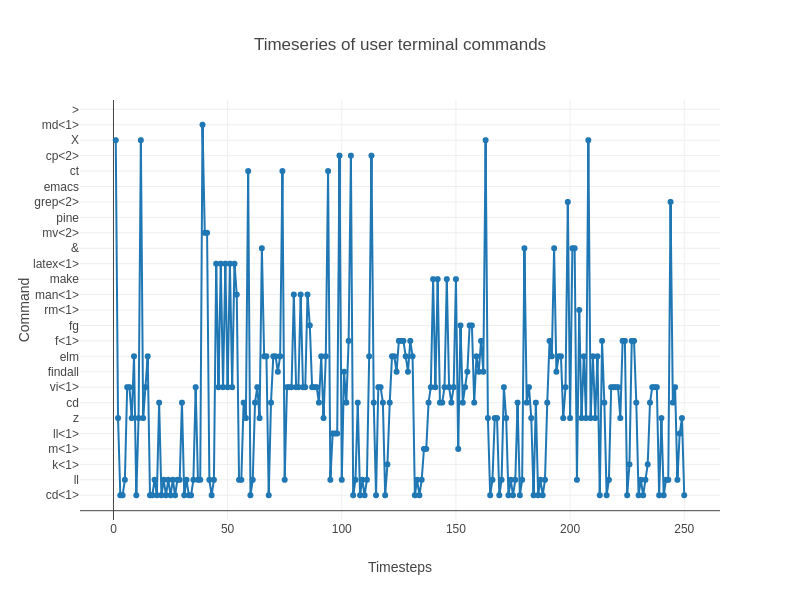
\includegraphics[scale=.50]{../pictures/250-empirical-timesteps.png}
\end{figure}

We plotted the entire time series and the first 250 steps. As the entire time series is very wild, we include the $250$ step one for analysis.

Also, note for the timeseries plot (on $250$ steps) how there are several back and forths between states; i.e. when trying to solve a problem usually alternating between two commands (ignoring other sparsely used commands) usually does the trick.
As an example, consider \texttt{cd} and \texttt{ll} (note this happens quite a bit in the chain).
If I am navigating around a coding project looking for files,
I will alternate between moving to a new directory (\texttt{cd}) and looking at the files in that directory (\texttt{ll}) to see where to go next.
Once I've found my file, I'll switch to another command such as the text editor.

As another example, switching between \texttt{vi}, i.e. text editting, and \texttt{latex} or \texttt{make} (which builds code) is also a common occurence.

\begin{figure}[!htb]
  \centering
  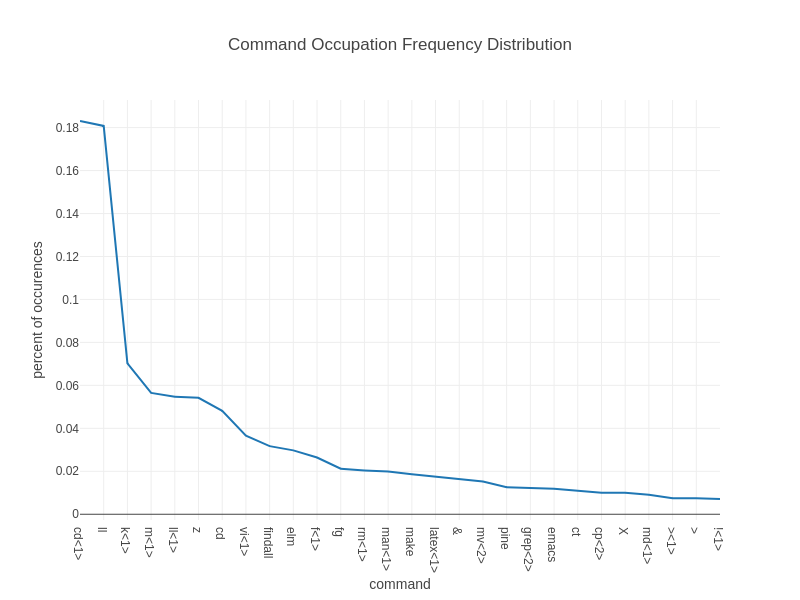
\includegraphics[scale=.50]{../pictures/empirical-occ-freq-dist.png}
\end{figure}

We calculated the occupation frequencies of the emperical data by counting the number of times each state was visited and graphed the
distribution. 

Even though the data is from 1998 the top 5 commands seem reasonable given our
own experience using UNIX based operating systems. The majority of the time a
user will be navigating their computer's file directory with commands like
\texttt{cd} and \texttt{ll}. \texttt{cd<1>} navigates to the given directory,
while \texttt{ll} gives a detailed description of files in current directory (name, owner, modified date, size, etc.).
Other common commands include \texttt{rm}, \texttt{cp}, and \text{mv} for file manipulation,
\texttt{grep} for searching, \texttt{latex} for latex,
and \texttt{emacs} and \texttt{vi} for text editting.

\begin{figure}[!htb]
  \centering
  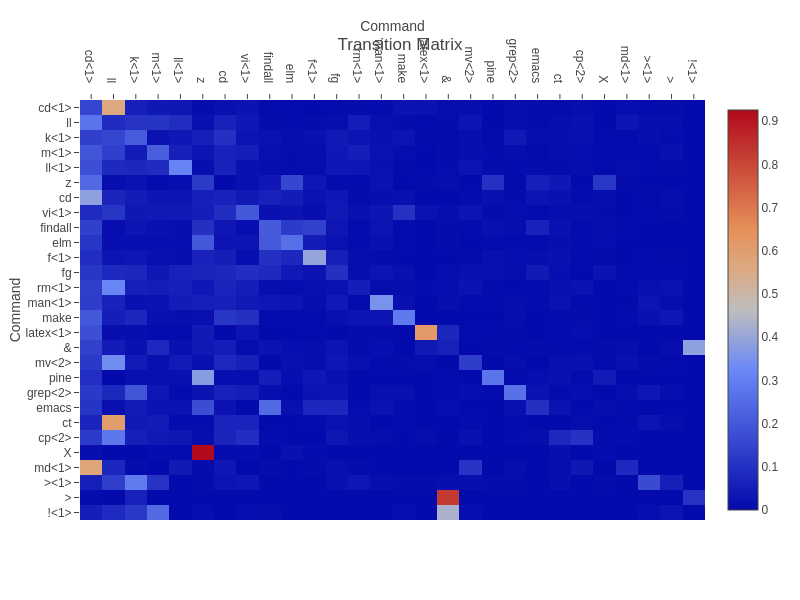
\includegraphics[scale=.60]{../pictures/transition-matrix-heatmap.png}
\end{figure}

Next we computed the transition matrix by counting the number of times the chain
went from state $i$ to state $j$ followed by dividing each count $P_{ij}$ by the
number of times we moved out of state $i$. 

We plotted the transition matrix as a heatmap, as we believe that this provides a much better understanding of the transitions of the chain. 

Note the high(er) frequency of the diagonal; after typing a command, you are more likely to type it again that typing most others.
Additionally, the column for \texttt{cd<1>} is brighter than most; after every command you are decently likely to navigate to another directory. 

We raised the transition matrix to the power $1000$ to compute the stationary
distribution. We argue that the original chain is irreducible because the data tracks the
user's usage of the UNIX machine over two years. This means that there are many
instances of logging in and out of the machine, which is done with the same set
of commands every time (\texttt{rlogin} and \texttt{exit}). So the only instance
where a state $i$ is unreachable from $j$ is if the user types a command and
then doesn't proceed to logoff or doesn't proceed to log on.

Both cases are impossible because a command isn't tracked until the user has logged on and
since we're tracking the $28$ most common commands there is no way that one of
these commands are used so frequently while the user never exit afterwrods.
Therefore, since the chain always visits the state \texttt{exit} every state can
reach \texttt{exit} and as a result every state can reach every other state via
the \texttt{exit} state.

Additionally, as there are no $0$ entries in the transition matrix to the $1000^{th}$ power, our cleaned chain is irreducible.

Therefore our stationary distribution is unique and when we plot it
against the occupation frequency distribution, there is no surprise that the
distributions are identical. The plot of the comparison is in the Appendix.

\begin{figure}[!htb]
  \centering
  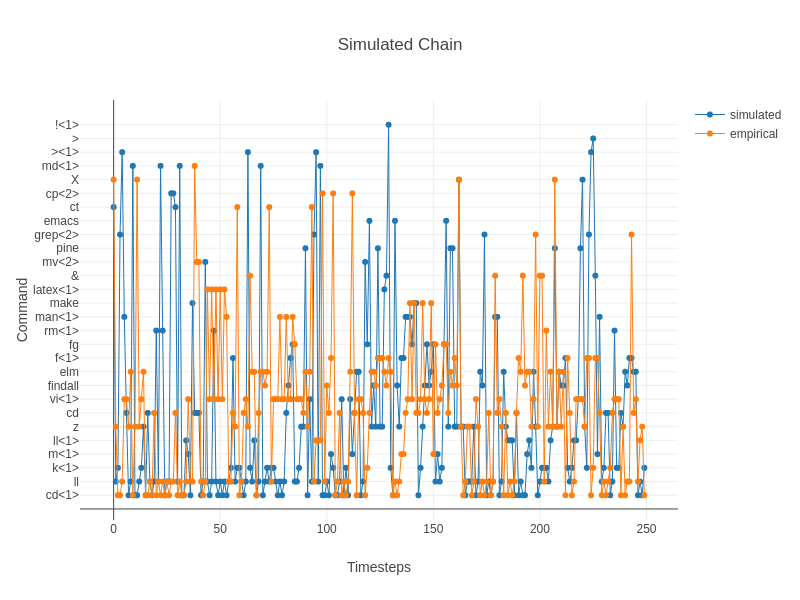
\includegraphics[scale=.55]{../pictures/simul-chain-vs-empirical-chain.png}
\end{figure}

We simluated the chain for $250$ time steps (it is too wild to get meaningful images with any more).
We chose the initial state uniformly randomly over all $28$.

Note how the original chain has many back and forths between lesser (i.e. not \texttt{cd} and \texttt{ll}) states, as discussed earlier,
while the simulated chain does not appear to capture this behavior.
In general, the simulated chain appears to lose much of the structure of the original chain,
bobbing around meaninglessly between states while the original chain has reoccuring patterns (though still with meaningless jumps up to less used states).

We made some attempts to display what happens in the chain clearer (as our states do not have any notion of continuity between them) but were unable to find a good visualization technique besides the scatter plot.

Finally we investigated the mixing time of the chain. We did this by, at each
time step, computing the occupation frequency of the chain from the first to the
current time step. At each step we calculate the occupational frequency of the
states seen so far and subtracted this distribution with the calculated
stationary distribution. We then plotted the $L_1$ norm of the difference.

After $900$ steps it has a different of around $0.1$, which is quite small. The chain gets to a difference of $0.5$ after only $50$. The chain appears to converge quite rapidly to the stationary distribution

\begin{figure}[!htb]
  \centering
  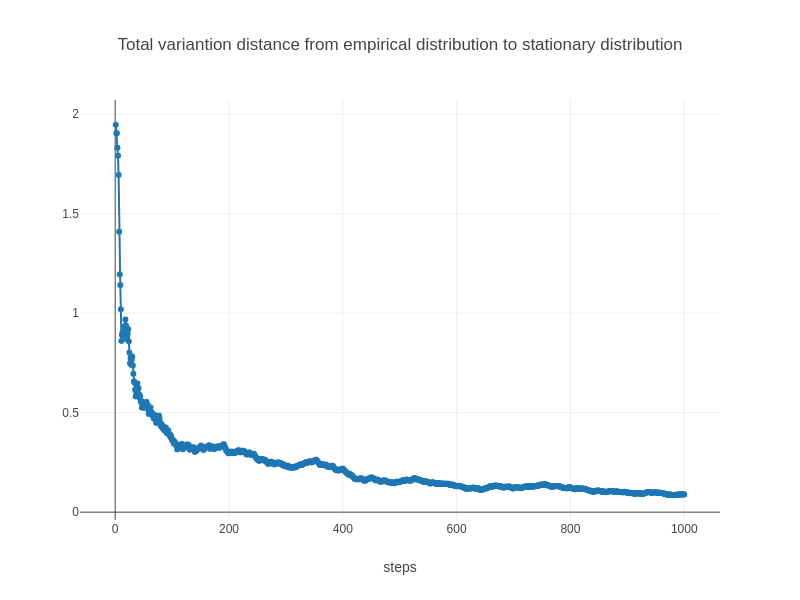
\includegraphics[scale=.45]{../pictures/mixing-time-analysis.png}
\end{figure}

\clearpage

\section{Appendix}

\begin{figure}[!htb]
  \centering
  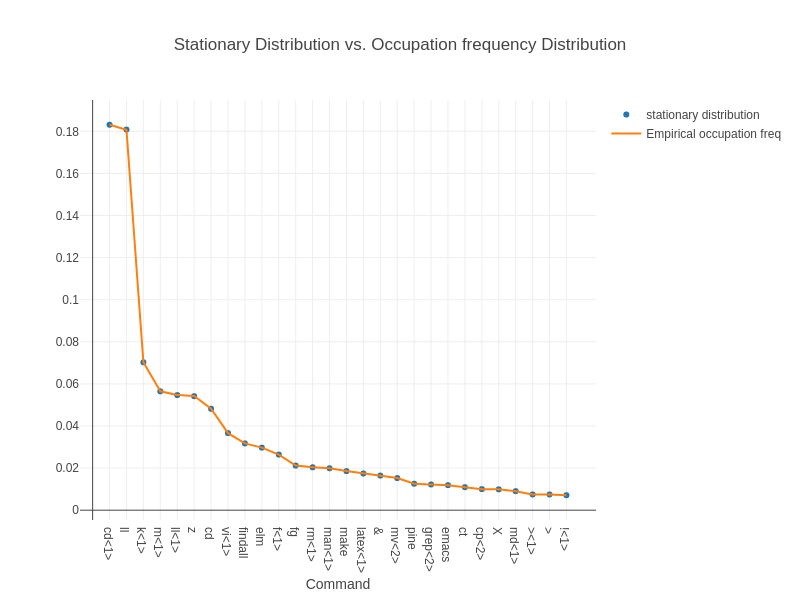
\includegraphics[scale=.50]{../pictures/stat-dist-and-empirical-occ-freq-dist.png}
\end{figure}

\end{document}

